% !TeX program = xelatex
\documentclass[a4paper,10pt]{article}

% ============================================================================
% កញ្ចប់បណ្ណាល័យ (Packages) – តាមលំនាំស្តង់ដារ អនុវិទ្យាល័យព្រះក្រសាំង (ls_plan.tex)
% បរិបទ៖ ថ្នាក់រៀនគ្មានស្លាយ LCD – បង្រៀនដោយប្រើក្ដារខៀន និងសន្លឹកកិច្ចការសិស្សស-ខ្មៅជាគោល
% ============================================================================
\usepackage[a4paper, left=0.95cm, right=0.95cm, top=0.85cm, bottom=0.92cm, footskip=0.52cm]{geometry}
\usepackage{amsmath}
\usepackage{unicode-math}
\usepackage{fontspec}
\usepackage{array, longtable, multirow, colortbl}
\usepackage[table]{xcolor}
\usepackage{enumitem}
\usepackage{pifont}
\usepackage{fancyhdr}
\usepackage{tikz}
\usetikzlibrary{calc, arrows.meta, angles, quotes, decorations.markings, positioning, babel}

\makeatletter
\let\@expl@@@mark@update@singlecol@structures@@\relax
\makeatother

% ============================================================================
% ការកំណត់ពុម្ពអក្សរផ្លូវការ (Cross-Platform Fonts Configuration)
% ============================================================================
\providecommand{\NGSFindFonts}{%
  \IfFileExists{C:/Windows/Fonts/cambria.ttc}{%
    \def\NGSSysPath{C:/Windows/Fonts/}%
    \def\NGSUserPath{C:/Users/KIT/AppData/Local/Microsoft/Windows/Fonts/}%
  }{%
    \IfFileExists{./fonts/KhmerOSsiemreap.ttf}{\def\NGSSysPath{./fonts/}\def\NGSUserPath{./fonts/}}{%
    \IfFileExists{../fonts/KhmerOSsiemreap.ttf}{\def\NGSSysPath{../fonts/}\def\NGSUserPath{../fonts/}}{%
    \IfFileExists{../../fonts/KhmerOSsiemreap.ttf}{\def\NGSSysPath{../../fonts/}\def\NGSUserPath{../../fonts/}}{%
    \IfFileExists{../../../fonts/KhmerOSsiemreap.ttf}{\def\NGSSysPath{../../../fonts/}\def\NGSUserPath{../../../fonts/}}{%
    \IfFileExists{../../../../fonts/KhmerOSsiemreap.ttf}{\def\NGSSysPath{../../../../fonts/}\def\NGSUserPath{../../../../fonts/}}{%
    \IfFileExists{../../../../../fonts/KhmerOSsiemreap.ttf}{\def\NGSSysPath{../../../../../fonts/}\def\NGSUserPath{../../../../../fonts/}}{%
    \IfFileExists{../../../../../../fonts/KhmerOSsiemreap.ttf}{\def\NGSSysPath{../../../../../../fonts/}\def\NGSUserPath{../../../../../../fonts/}}{%
      \def\NGSSysPath{../../../../../../../fonts/}\def\NGSUserPath{../../../../../../../fonts/}%
    }}}}}}}%
  }%
}
\NGSFindFonts

\setmathfont[Path={\NGSSysPath}, FontIndex=1, Scale=1.02]{cambria.ttc}
\defaultfontfeatures{Ligatures=TeX}

\setmainfont[
  Path={\NGSUserPath},
  Extension=.ttf,
  Script=Khmer,
  BoldFont={KhmerOSsiemreap},
  BoldFeatures={FakeBold=1.8},
  ItalicFont={KhmerOSsiemreap},
  ItalicFeatures={FakeSlant=0.25},
  BoldItalicFont={KhmerOSsiemreap},
  BoldItalicFeatures={FakeBold=1.8, FakeSlant=0.25}
]{KhmerOSsiemreap}

\newfontfamily\muol[Path={\NGSUserPath}, Extension=.ttf, Script=Khmer]{KhmerOSmuollight}
\newfontfamily\TimesEn[Path={\NGSSysPath}, Extension=.ttf, BoldFont={timesbd}, ItalicFont={timesi}, BoldItalicFont={timesbi}]{times}
\newfontfamily\NagaBold[Path={\NGSUserPath}, Extension=.ttf]{AKbalthom Naga Bold}
\newfontfamily\CalibriFont[Path={\NGSSysPath}, Extension=.ttf]{calibri}
\newfontfamily\Tacteing[Path={\NGSUserPath}]{TACTENG.TTF}
\newfontfamily\CourierBullet[Path={\NGSSysPath}, Extension=.ttf]{cour}
\newcommand{\wcirc}{{\CourierBullet\fontsize{9.5pt}{11pt}\selectfont o}}

\XeTeXlinebreaklocale "km"
\XeTeXlinebreakskip = 0pt plus 1pt minus 0.1pt

\definecolor{stepgray}{HTML}{D9D9D9}
\definecolor{headgray}{HTML}{F2F2F2}
\definecolor{boxgray}{HTML}{D9D9D9}
\definecolor{darkred}{HTML}{C00000}
\definecolor{red5e}{HTML}{FF0000}

\pagestyle{fancy}
\fancyhf{}
\renewcommand{\headrulewidth}{0pt}
\fancyfoot[R]{\CalibriFont\fontsize{11pt}{13pt}\selectfont\thepage}

\setlength{\parindent}{0pt}
\setlength{\parskip}{0pt}
\setlength{\tabcolsep}{3.8pt}

\newcolumntype{L}[1]{>{\raggedright\arraybackslash}p{#1}}

\newcommand{\en}[1]{{\TimesEn #1}}
\newcommand{\enbf}[1]{{\TimesEn\textbf{#1}}}
\newcommand{\unit}[1]{\,\text{\en{#1}}}
\newcommand{\fiveE}[1]{{\NagaBold\fontsize{9.5pt}{13pt}\selectfont\textcolor{red5e}{#1}}}
\newcommand{\timenote}[1]{\textcolor{darkred}{\textit{#1}}}
\newcommand{\redsub}[1]{\textcolor{darkred}{#1}}
\newcommand{\graybox}[1]{\colorbox{boxgray}{\strut\hspace{2pt}#1\hspace{2pt}}}
\newcommand{\ditem}{\tikz[baseline=-0.5ex]\fill (0,0.42ex) -- (0.42ex,0) -- (0,-0.42ex) -- (-0.42ex,0) -- cycle;\hspace{0.3em}}
\newcommand{\cnum}[1]{{\fontsize{10.5pt}{12pt}\selectfont\ding{\numexpr171+#1\relax}}\hspace{0.2em}}
\newcommand{\cfig}[1]{\par\vspace{4pt}{\centering #1\par}\vspace{4pt}}
\newcommand{\stepheader}[1]{\multicolumn{3}{|c|}{\cellcolor{stepgray}\muol #1} \\* \noalign{\hrule height 0.4pt}}
\newcommand{\tri}[1]{\ensuremath{\triangle #1}}
\newcommand{\ang}[1]{\ensuremath{\angle #1}}
\newcommand{\cg}{\ensuremath{\cong}}
\newcommand{\khmflourish}{{\Tacteing\fontsize{36pt}{14pt}\selectfont\raisebox{-5pt}{3}}}

\tikzset{
  tk1/.style={postaction={decorate},decoration={markings,mark=at position 0.50 with {\draw[black, line width=0.85pt](0,-0.095)--(0,0.095);}}},
  tk2/.style={postaction={decorate},decoration={markings,
    mark=at position 0.45 with {\draw[black, line width=0.85pt](0,-0.095)--(0,0.095);},
    mark=at position 0.55 with {\draw[black, line width=0.85pt](0,-0.095)--(0,0.095);}}},
  tk3/.style={postaction={decorate},decoration={markings,
    mark=at position 0.42 with {\draw[black, line width=0.85pt](0,-0.095)--(0,0.095);},
    mark=at position 0.50 with {\draw[black, line width=0.85pt](0,-0.095)--(0,0.095);},
    mark=at position 0.58 with {\draw[black, line width=0.85pt](0,-0.095)--(0,0.095);}}},
  par1/.style={postaction={decorate},decoration={markings,mark=at position 0.52 with {\draw[black, line width=0.85pt](-0.07,0.08)--(0.05,0)--(-0.07,-0.08);}}},
  par2/.style={postaction={decorate},decoration={markings,
    mark=at position 0.46 with {\draw[black, line width=0.85pt](-0.07,0.08)--(0.05,0)--(-0.07,-0.08);},
    mark=at position 0.58 with {\draw[black, line width=0.85pt](-0.07,0.08)--(0.05,0)--(-0.07,-0.08);}}}
}

% ============================================================================
% ម៉ាក្រូរូបភាពធរណីមាត្រស-ខ្មៅ (Proportional 4.0–7.2 cm B&W TikZ Diagrams)
% ============================================================================

% ១. រំលឹកមេរៀនទាក់ទង៖ លក្ខណៈប្រលេឡូក្រាម + ត្រីកោណកែងប៉ុនគ្នា (ជ-ម-ជ / ជ-ជ-ជ)
\newcommand{\figPrereqRECT}{%
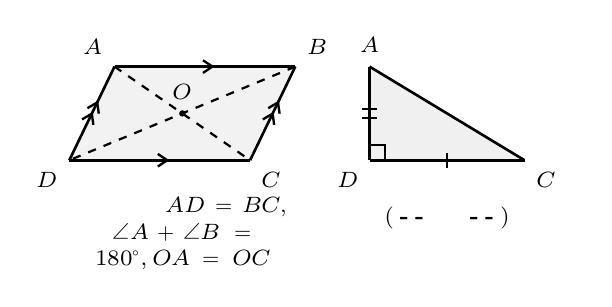
\begin{tikzpicture}[scale=0.82, every node/.style={font=\footnotesize, text=black}]
  % ឆ្វេង៖ ប្រលេឡូក្រាមទូទៅ
  \begin{scope}[shift={(0,0)}]
    \coordinate (D) at (0,0); \coordinate (C) at (2.8,0);
    \coordinate (A) at (0.7,1.45); \coordinate (B) at (3.5,1.45);
    \coordinate (O) at ($(A)!0.5!(C)$);
    \fill[gray!10] (A)--(B)--(C)--(D)--cycle;
    \draw[black, line width=0.95pt, par1] (A)--(B); \draw[black, line width=0.95pt, par1] (D)--(C);
    \draw[black, line width=0.95pt, par2] (D)--(A); \draw[black, line width=0.95pt, par2] (C)--(B);
    \draw[black, line width=0.8pt, dashed] (A)--(C) (B)--(D);
    \fill[black] (O) circle (1.4pt) node[above=1.5pt] {$O$};
    \node[above left=1pt] at (A) {$A$}; \node[above right=1pt] at (B) {$B$};
    \node[below right=1pt] at (C) {$C$}; \node[below left=1pt] at (D) {$D$};
    \node[anchor=north, text width=3.35cm, align=center] at (1.75,-0.42) {ប្រលេឡូក្រាម៖ $AD=BC$,\\$\ang{A}+\ang{B}=180^\circ, OA=OC$};
  \end{scope}
  % ស្ដាំ៖ ត្រីកោណកែងប៉ុនគ្នា
  \begin{scope}[shift={(4.65,0)}]
    \coordinate (D) at (0,0); \coordinate (C) at (2.4,0); \coordinate (A) at (0,1.45);
    \fill[gray!12] (D)--(C)--(A)--cycle;
    \draw[black, line width=0.95pt, tk2] (D)--(A);
    \draw[black, line width=0.95pt, tk1] (D)--(C);
    \draw[black, line width=0.95pt] (A)--(C);
    \draw[black, line width=0.75pt] (0,0.24)--(0.24,0.24)--(0.24,0);
    \node[above=1.5pt] at (A) {$A$}; \node[below left=1pt] at (D) {$D$}; \node[below right=1pt] at (C) {$C$};
    \node[anchor=north, text width=3.25cm, align=center] at (1.20,-0.42) {ត្រីកោណកែងប៉ុនគ្នា\\(\textbf{ជ-ម-ជ} និង \textbf{ជ-ជ-ជ})};
  \end{scope}
\end{tikzpicture}}

% ២. E1 Engage: វិធីវាស់ខ្សែទ្រូងស៊ុមបង្អួចរបស់ជាងឈើ ទល់នឹង អន្ទាក់ចតុកោណព្នាយសមបាត
\newcommand{\figEngageRECT}{%
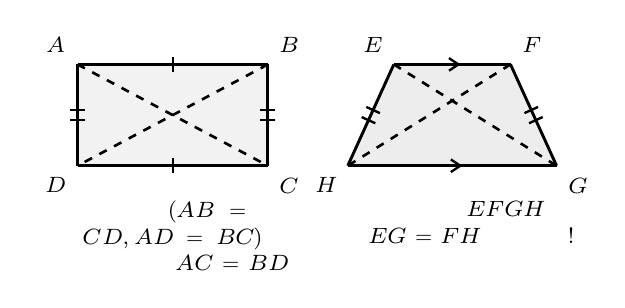
\begin{tikzpicture}[scale=0.78, every node/.style={font=\footnotesize, text=black}]
  % ឆ្វេង៖ ស៊ុមបង្អួចប្រលេឡូក្រាម (AB=CD, AD=BC) វាស់ AC = BD
  \begin{scope}[shift={(0,0)}]
    \coordinate (D) at (0,0); \coordinate (C) at (3.10,0);
    \coordinate (A) at (0,1.65); \coordinate (B) at (3.10,1.65);
    \fill[gray!10] (A)--(B)--(C)--(D)--cycle;
    \draw[black, line width=1.05pt, tk1] (A)--(B); \draw[black, line width=1.05pt, tk1] (D)--(C);
    \draw[black, line width=1.05pt, tk2] (D)--(A); \draw[black, line width=1.05pt, tk2] (C)--(B);
    \draw[black, line width=0.95pt, dashed] (A)--(C) (B)--(D);
    \node[above left=1pt] at (A) {$A$}; \node[above right=1pt] at (B) {$B$};
    \node[below right=1pt] at (C) {$C$}; \node[below left=1pt] at (D) {$D$};
    \node[anchor=north, text width=3.45cm, align=center] at (1.55,-0.42) {ស៊ុមបង្អួច ($AB=CD, AD=BC$)\\ជាងឈើវាស់ខ្សែទ្រូង $AC = BD$};
  \end{scope}
  % ស្ដាំ៖ ចតុកោណព្នាយសមបាត ក៏មានអង្កត់ទ្រូងស្មើគ្នាដែរ!
  \begin{scope}[shift={(4.40,0)}]
    \coordinate (H) at (0,0); \coordinate (G) at (3.40,0);
    \coordinate (E) at (0.75,1.65); \coordinate (F) at (2.65,1.65);
    \fill[gray!14] (E)--(F)--(G)--(H)--cycle;
    \draw[black, line width=1.05pt, par1] (E)--(F); \draw[black, line width=1.05pt, par1] (H)--(G);
    \draw[black, line width=1.05pt, tk2] (H)--(E); \draw[black, line width=1.05pt, tk2] (G)--(F);
    \draw[black, line width=0.95pt, dashed] (E)--(G) (F)--(H);
    \node[above left=1pt] at (E) {$E$}; \node[above right=1pt] at (F) {$F$};
    \node[below right=1pt] at (G) {$G$}; \node[below left=1pt] at (H) {$H$};
    \node[anchor=north, text width=3.45cm, align=center] at (1.70,-0.42) {ចតុកោណព្នាយសមបាត $EFGH$\\ក៏មាន $EG = FH$ តែមុំមិនកែងទេ!};
  \end{scope}
\end{tikzpicture}}

% ៣. E2/E3: ការបំបែកត្រីកោណត្រួតគ្នា \triangle ADC & \triangle BDC (Duval Deconstruction)
\newcommand{\figDeconstructRECT}{%
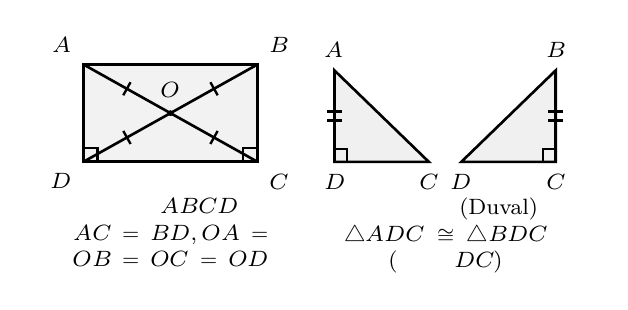
\begin{tikzpicture}[scale=0.75, every node/.style={font=\footnotesize, text=black}]
  % ឆ្វេង៖ រូបដើមចតុកោណកែង ABCD មានអង្កត់ទ្រូងត្រួតគ្នា
  \begin{scope}[shift={(0,0)}]
    \coordinate (D) at (0,0); \coordinate (C) at (2.95,0);
    \coordinate (A) at (0,1.65); \coordinate (B) at (2.95,1.65);
    \coordinate (O) at (1.475,0.825);
    \fill[gray!10] (A)--(B)--(C)--(D)--cycle;
    \draw[black, line width=1.0pt] (A)--(B)--(C)--(D)--cycle;
    \draw[black, line width=0.95pt, tk1] (A)--(O); \draw[black, line width=0.95pt, tk1] (O)--(C);
    \draw[black, line width=0.95pt, tk1] (B)--(O); \draw[black, line width=0.95pt, tk1] (O)--(D);
    \draw[black, line width=0.75pt] (0,0.24)--(0.24,0.24)--(0.24,0);
    \draw[black, line width=0.75pt] (2.71,0)--(2.71,0.24)--(2.95,0.24);
    \fill[black] (O) circle (1.4pt) node[above=2pt] {$O$};
    \node[above left=1pt] at (A) {$A$}; \node[above right=1pt] at (B) {$B$};
    \node[below right=1pt] at (C) {$C$}; \node[below left=1pt] at (D) {$D$};
    \node[anchor=north, text width=3.40cm, align=center] at (1.48,-0.45) {ចតុកោណកែង $ABCD$៖\\$AC=BD, OA=OB=OC=OD$};
  \end{scope}
  % ស្ដាំ៖ បំបែកត្រីកោណត្រួតគ្នា \triangle ADC និង \triangle BDC ដាច់ពីគ្នា
  \begin{scope}[shift={(4.25,0)}]
    % \triangle ADC
    \draw[black, line width=0.95pt, fill=gray!12] (0,0)--(1.60,0)--(0,1.55)--cycle;
    \draw[black, line width=0.95pt, tk2] (0,0)--(0,1.55);
    \draw[black, line width=0.7pt] (0,0.22)--(0.22,0.22)--(0.22,0);
    \node[above=1pt] at (0,1.55) {$A$}; \node[below=1pt] at (0,0) {$D$}; \node[below=1pt] at (1.60,0) {$C$};
    % \triangle BDC
    \begin{scope}[shift={(2.15,0)}]
      \draw[black, line width=0.95pt, fill=gray!12] (0,0)--(1.60,0)--(1.60,1.55)--cycle;
      \draw[black, line width=0.95pt, tk2] (1.60,0)--(1.60,1.55);
      \draw[black, line width=0.7pt] (1.38,0)--(1.38,0.22)--(1.60,0.22);
      \node[above=1pt] at (1.60,1.55) {$B$}; \node[below=1pt] at (0,0) {$D$}; \node[below=1pt] at (1.60,0) {$C$};
    \end{scope}
    \node[anchor=north, text width=3.70cm, align=center] at (1.88,-0.45) {បំបែករូបត្រួតគ្នា (\en{Duval})៖\\$\tri{ADC}\cg\tri{BDC}$ (ជ្រុងរួម $DC$)};
  \end{scope}
\end{tikzpicture}}

% ៤. E4 Elaborate: គំរូទី១ (លំហាត់ទី៩ ទំ.១៨៦) & គំរូទី២ (លំហាត់គំរូ ទំ.១៧៦ MP+MQ=BH)
\newcommand{\figModelRECT}{%
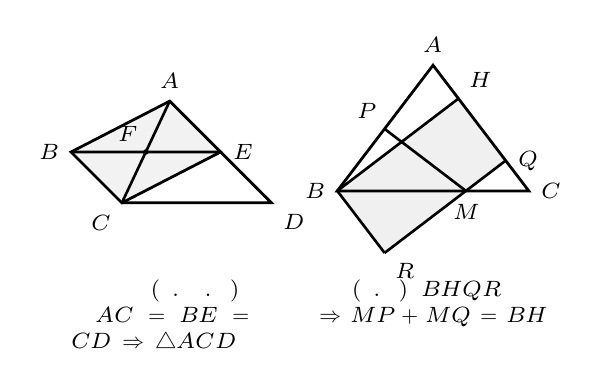
\begin{tikzpicture}[scale=0.76, every node/.style={font=\footnotesize, text=black}]
  % ឆ្វេង៖ លំហាត់ទី៩ ទំ.១៨៦ (ចតុកោណកែង ABCE & ប្រលេឡូក្រាម BCDE, ស្របតាមរូបសៀវភៅគោល)
  \begin{scope}[shift={(0,0.15)}]
    \coordinate (C) at (0.85,0);
    \coordinate (D) at (3.35,0);
    \coordinate (B) at (0,0.85);
    \coordinate (E) at (2.50,0.85);
    \coordinate (A) at (1.65,1.70);
    \coordinate (F) at ($(A)!0.5!(C)$);
    \fill[gray!10] (A)--(B)--(C)--(E)--cycle;
    \draw[black, line width=1.0pt] (A)--(B)--(C)--(E)--cycle;
    \draw[black, line width=1.0pt] (C)--(D)--(E);
    \draw[black, line width=0.95pt] (A)--(C) (B)--(E);
    \draw[black, line width=0.85pt, dashed] (A)--(D);
    \fill[black] (F) circle (1.3pt) node[above left=0.5pt] {$F$};
    \node[above=1pt] at (A) {$A$}; \node[left=1pt] at (B) {$B$};
    \node[below left=1pt] at (C) {$C$}; \node[below right=1pt] at (D) {$D$};
    \node[right=1pt] at (E) {$E$};
    \node[anchor=north, text width=3.45cm, align=center] at (1.70,-1.12) {គំរូទី១ (លំ.៩ ទំ.១៨៦)៖\\$AC=BE=CD \Rightarrow \tri{ACD}$ សមបាត};
  \end{scope}
  % ស្ដាំ៖ លំហាត់គំរូ ទំ.១៧៦ (ត្រីកោណសមបាត ABC, BHQR ជាចតុកោណកែង => MP+MQ=BH)
  \begin{scope}[shift={(4.45,0.35)}]
    \coordinate (B) at (0,0);
    \coordinate (C) at (3.20,0);
    \coordinate (A) at (1.60,2.10);
    \coordinate (M) at (2.15,0);
    \coordinate (P) at ($(A)!(M)!(B)$);
    \coordinate (Q) at ($(A)!(M)!(C)$);
    \coordinate (H) at ($(A)!(B)!(C)$);
    \path let \p1 = ($(M)-(P)$), \p2 = ($(M)-(Q)$),
              \n1 = {veclen(\x1,\y1)}, \n2 = {veclen(\x2,\y2)} in
          coordinate (R) at ($(M) + {\n1/\n2}*($(M)-(Q)$)$);
    \fill[gray!12] (B)--(H)--(Q)--(R)--cycle;
    \draw[black, line width=1.0pt] (A)--(B)--(C)--cycle;
    \draw[black, line width=0.95pt] (B)--(H) (M)--(P) (Q)--(R) (B)--(R);
    \node[above=1pt] at (A) {$A$}; \node[left=1pt] at (B) {$B$}; \node[right=1pt] at (C) {$C$};
    \node[above left=0.5pt] at (P) {$P$}; \node[above right=0.5pt] at (H) {$H$};
    \node[right=1pt] at (Q) {$Q$}; \node[below=1.5pt] at (M) {$M$}; \node[below right=0.5pt] at (R) {$R$};
    \node[anchor=north, text width=3.45cm, align=center] at (1.60,-1.32) {គំរូទី២ (ទំ.១៧៦)៖ $BHQR$ ចតុកោណកែង\\$\Rightarrow MP + MQ = BH$};
  \end{scope}
\end{tikzpicture}}

% ៥. E5 Evaluate: ប្រតិបត្តិ ទំ.១៧៦ (ចតុកោណកែង ABCD => \angle CAD = \angle BDA)
\newcommand{\figPractRECT}{%
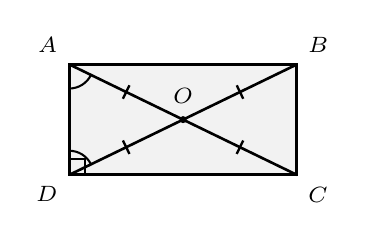
\begin{tikzpicture}[scale=0.85, every node/.style={font=\footnotesize, text=black}]
  \coordinate (D) at (0,0); \coordinate (C) at (3.40,0);
  \coordinate (A) at (0,1.65); \coordinate (B) at (3.40,1.65);
  \coordinate (O) at (1.70,0.825);
  \fill[gray!10] (A)--(B)--(C)--(D)--cycle;
  \draw[black, line width=1.0pt] (A)--(B)--(C)--(D)--cycle;
  \draw[black, line width=0.95pt, tk1] (A)--(O); \draw[black, line width=0.95pt, tk1] (O)--(D);
  \draw[black, line width=0.95pt, tk1] (B)--(O); \draw[black, line width=0.95pt, tk1] (O)--(C);
  \draw[black, line width=0.75pt] (0,0.24)--(0.24,0.24)--(0.24,0);
  \draw[black, line width=0.75pt] ($(A)+(-90:0.36)$) arc (-90:-26:0.36);
  \draw[black, line width=0.75pt] ($(D)+(90:0.36)$) arc (90:26:0.36);
  \fill[black] (O) circle (1.5pt) node[above=2pt] {$O$};
  \node[above left=1pt] at (A) {$A$}; \node[above right=1pt] at (B) {$B$};
  \node[below right=1pt] at (C) {$C$}; \node[below left=1pt] at (D) {$D$};
\end{tikzpicture}}

\begin{document}
\fontsize{10pt}{15.2pt}\selectfont

% -------------------- ក្បាលកិច្ចតែងការ (Header) --------------------
\begin{center}
  {\muol\fontsize{11pt}{16pt}\selectfont ព្រះរាជាណាចក្រកម្ពុជា}\\[2pt]
  {\muol\fontsize{10pt}{15pt}\selectfont ជាតិ សាសនា ព្រះមហាក្សត្រ}\\[1pt]
  \khmflourish
\end{center}

\vspace{-28pt}
{\muol\fontsize{9.5pt}{12.5pt}\selectfont
មន្ទីរអប់រំ យុវជន និងកីឡា ខេត្តកំពង់ធំ\\
ការិយាល័យអប់រំ យុវជន និងកីឡា ស្រុកកំពង់ស្វាយ\\
អនុវិទ្យាល័យព្រះក្រសាំង}

\vspace{1pt}
\begin{center}
  {\muol\fontsize{10pt}{14pt}\selectfont កិច្ចតែងការបង្រៀន}
\end{center}
\vspace{0pt}

% -------------------- ព័ត៌មានទូទៅ (Metadata) --------------------
{\renewcommand{\arraystretch}{0.95}
\hspace*{4.05cm}%
\begin{tabular}{@{}l l l@{}}
  - \hspace{0.35cm} មុខវិជ្ជា & : & គណិតវិទ្យា ថ្នាក់ទី៨ \\
  - \hspace{0.35cm} ចំណងជើងមេរៀន & : & មេរៀនទី១៣ ចតុកោណ \\
  - \hspace{0.35cm} ចំណងជើងរង & : & ២.២ លក្ខណៈចតុកោណកែង (ទំ.១៧៤--១៧៦ និងទំ.១៨៦) \\
  - \hspace{0.35cm} រយៈពេល & : & ១ ម៉ោងសិក្សា (៥០ នាទី) \\
  - \hspace{0.35cm} បង្រៀនដោយ & : & ហុក ប៊ុនថែន \\
  - \hspace{0.35cm} កាលបរិច្ឆេទ & : & ថ្ងៃអង្គារ ៦កើត ខែមិគសិរ ព.ស.២៥៧០ (១៥ ធ្នូ ២០២៦) \\
\end{tabular}

\vspace{1pt}

% -------------------- I. វត្ថុបំណង --------------------
\textbf{I.} {\muol វត្ថុបំណង}\\[1pt]
\hspace*{0.55cm}%
\begin{tabular}{@{}l l L{14.2cm}@{}}
  \wcirc \hspace{0.25cm} វិជ្ជាសម្បទា & : & សិស្សពោលបានត្រឹមត្រូវនូវនិយមន័យចតុកោណកែង (ប្រលេឡូក្រាមមានមុំកែងមួយ) ទ្រឹស្ដីបទទី១ (មុំទាំងបួនជាមុំកែង) ទ្រឹស្ដីបទទី២ និងវិបាក (អង្កត់ទ្រូងប៉ុនគ្នា និងចែកជាបួនកំណាត់ស្មើគ្នា $OA=OB=OC=OD$) ព្រមទាំងទ្រឹស្ដីបទទី៣ (ប្រលេឡូក្រាមមានអង្កត់ទ្រូងប៉ុនគ្នាជាចតុកោណកែង) តាមសៀវភៅគោល ទំ.១៧៤--១៧៦ ។ \\
  \wcirc \hspace{0.25cm} បំណិនសម្បទា & : & សិស្សបំបែកត្រីកោណកែងត្រួតគ្នា ($\tri{ADC}$ និង $\tri{BDC}$) លើសន្លឹកកិច្ចការស-ខ្មៅ ដើម្បីស្រាយបញ្ជាក់ទ្រឹស្ដីបទទី២--៣ ព្រមទាំងដោះស្រាយលំហាត់សម្រាយបញ្ជាក់ និងគណនាប្រវែងអង្កត់ទ្រូង-មុំដោយភ្ជាប់ធនាគារហេតុផល \cnum{1}--\cnum{5} ។ \\
  \wcirc \hspace{0.25cm} ចរិយាសម្បទា & : & សិស្សមានទម្លាប់ពិនិត្យលក្ខខណ្ឌប្រលេឡូក្រាមមុនសន្និដ្ឋានតាមអង្កត់ទ្រូងស្មើគ្នា (មិនច្រឡំនឹងចតុកោណព្នាយសមបាត ឬច្រឡំថាអង្កត់ទ្រូងចតុកោណកែងពុះមុំកែងជា $45^\circ$ ឡើយ) និងផ្សារភ្ជាប់ទៅនឹងបច្ចេកទេសជាងឈើវាស់ជ្រុងកែងស៊ុមបង្អួច ។ \\
\end{tabular}

\vspace{1pt}

% -------------------- II. សម្ភារៈឧបទេស --------------------
\textbf{II.} {\muol សម្ភារៈឧបទេស}\\[1pt]
\hspace*{0.55cm}$\bullet$ \hspace{0.35cm} សៀវភៅសិក្សាគោលគណិតវិទ្យាថ្នាក់ទី៨ (ទំ.១៧៤--១៧៦ និងទំ.១៨៦) ក្ដារខៀន ដីស បន្ទាត់ក្រិត រ៉ាប់ព័រទ័រ ដែកឈាន និងសន្លឹកកិច្ចការសិស្សស-ខ្មៅ (\en{Worksheet\_RECT1} ចំនួន ២ ទំព័រ \en{A4} ដោយគ្មានស្លាយ \en{LCD}) ។

\vspace{1pt}

% -------------------- III. វិធីសាស្រ្តបង្រៀន --------------------
\textbf{III.} {\muol វិធីសាស្រ្តបង្រៀន}\\[1pt]
\hspace*{0.45cm}%
\begin{tabular}{@{}l l L{14.85cm}@{}}
  $\bullet$ \hspace{0.25cm} គោលវិធី & : & សិស្សមជ្ឈមណ្ឌល (សិក្សាស៊ើបអង្កេតជាដៃគូលើសន្លឹកកិច្ចការបំពេញផ្ទាល់ គ្មានស្លាយ \en{LCD}) \\
  $\bullet$ \hspace{0.25cm} យុទ្ធវិធីបង្រៀន & : & គម្រូស្ថាបនានិយម \en{5Es} រួមបញ្ចូល \textbf{វិធីបំបែករូបត្រីកោណត្រួតស៊ីគ្នាដាច់ដោយឡែក} (\en{Duval Dimensional Deconstruction — Duval, 2006; Agostini et al., 2023}) \\
\end{tabular}
}

\vspace{1pt}

% -------------------- IV. ដំណើរការបង្រៀន --------------------
\textbf{IV.} {\muol ដំណើរការបង្រៀន}

\vspace{1pt}

\renewcommand{\arraystretch}{1.15}
\begin{longtable}{|L{5.50cm}|L{7.90cm}|L{4.80cm}|}
\hline
\rowcolor{headgray}
\multicolumn{1}{|c|}{\muol សកម្មភាពគ្រូ} &
\multicolumn{1}{c|}{\muol ខ្លឹមសារមេរៀន} &
\multicolumn{1}{c|}{\muol សកម្មភាពសិស្ស} \\
\hline
\endfirsthead
\hline
\endhead
\hline
\endfoot
\hline
\endlastfoot

% ==================== ជំហានទី១ (2min) ====================
\stepheader{ជំហានទី១ \enbf{(}រដ្ឋបាលថ្នាក់\enbf{)}}
$\bullet$ ពិនិត្យអវត្តមាន សណ្ដាប់ធ្នាប់ អនាម័យ និងសម្ភារៈធរណីមាត្រ (បន្ទាត់ក្រិត រ៉ាប់ព័រទ័រ ដែកឈាន)
&
$\bullet$ ពិនិត្យវត្តមាន និងសណ្ដាប់ធ្នាប់ថ្នាក់រៀន \par
$\bullet$ ត្រៀមបន្ទាត់ក្រិត និងរ៉ាប់ព័រទ័រសម្រាប់វាស់លើសន្លឹកកិច្ចការ
&
$\circ$ ប្រធានថ្នាក់រាយការណ៍អវត្តមាន និងត្រៀមឧបករណ៍ធរណីមាត្រ \\[3pt]

$\bullet$ រៀបចំសិស្សជាដៃគូពិភាក្សា រួចចែកសន្លឹកកិច្ចការ \en{Worksheet\_RECT1} (២ ទំព័រ \en{A4}) ផ្កាប់លើតុ
&
$\bullet$ ការចាត់ដៃគូសិក្សា និងចែកសន្លឹកកិច្ចការស-ខ្មៅ
&
$\circ$ អង្គុយតាមដៃគូ និងទទួលសន្លឹកកិច្ចការទុកលើតុ \\
\hline

% ==================== ជំហានទី២ (9min: <=3 + 3 + E1 3) ====================
\stepheader{ជំហានទី២ \enbf{(}កិច្ចការផ្ទះ \enbf{+} ទំនាក់ទំនងមេរៀនថ្មី\enbf{)}}
\ditem \textbf{កំណែកិច្ចការផ្ទះ ($\le 3\unit{min}$)} \timenote{សង្ខេបខ្លីលើក្ដារខៀន}
&
{\centering\redsub{កំណែកិច្ចការផ្ទះ (លំហាត់ទី៣ខ និងទី៧ ទំ.១៨៥)}\par}
&
$\circ$ យកសៀវភៅកិច្ចការផ្ទះមកផ្ទៀងផ្ទាត់ \\[2pt]

$\bullet$ ផ្ទៀងផ្ទាត់ចម្លើយលំហាត់ទី៣ខ និងលំហាត់ទី៧ យ៉ាងរហ័សលើក្ដារខៀន
&
$\bullet$ \textbf{លំ.៣ខ៖} $EH\parallel FI, EH=IF \Rightarrow EFIH$ ជាប្រលេឡូក្រាម ហើយ $FG=IF \Rightarrow \tri{FIG}$ ជាត្រីកោណសមបាតកំពូល $F$ ។ \par
$\bullet$ \textbf{លំ.៧៖} $OA'=OC', OB'=OD' \Rightarrow A'B'C'D'$ ជាប្រលេឡូក្រាម ។
&
$\circ$ ផ្ទៀងផ្ទាត់ចម្លើយ និងកែលម្អចំណុចខ្វះខាត \\[3pt]

\ditem \textbf{រំលឹកមេរៀនទាក់ទង ($3\unit{min}$)} \par
$\bullet$ គូសរូបលើក្ដារខៀន សួររំលឹក៖ បើប្រលេឡូក្រាម $ABCD$ មានមុំមួយ $\ang{A}=90^\circ$ តើមុំឈម $\ang{C}$ និងមុំជាប់ $\ang{B}, \ang{D}$ ស្មើប៉ុន្មាន?
&
{\centering\redsub{រំលឹកមេរៀនទាក់ទងមេរៀនថ្មី}\par} \par
$\bullet$ ក្នុងប្រលេឡូក្រាម៖ បើ $\ang{A}=90^\circ$ នោះមុំឈម $\ang{C}=90^\circ$ ហើយដោយ $\ang{A}+\ang{B}=180^\circ$ គេបាន $\ang{B}=\ang{D}=90^\circ$ ដែរ! \par
$\bullet$ លក្ខណៈត្រីកោណប៉ុនគ្នា \textbf{ជ-ម-ជ} និង \textbf{ជ-ជ-ជ} ។
&
$\circ$ គណនាផ្ទាល់មាត់៖ «មុំទាំងបួននឹងស្មើ $90^\circ$ ទាំងអស់!» និងរំលឹកលក្ខណៈត្រីកោណប៉ុនគ្នា \\[3pt]

&
\cfig{\figPrereqRECT}
& \\[3pt]

\fiveE{E1 - Engage (3min)} \timenote{(កុំទាន់ផ្ដល់ចម្លើយ)} \par
\ditem \textbf{បញ្ហាភ្ញាក់ផ្អើល «វិធីផ្ទៀងជ្រុងកែងស៊ុមបង្អួចដោយខ្សែពួរ»៖} \par
$\bullet$ លើកស្ថានភាពជាងឈើដំឡើងស៊ុមបង្អួច $ABCD$ ដែលកាត់ឈើឈមស្មើគ្នា ($AB=CD, AD=BC$) តែភ្លេចយកដែកកែងមកជាមួយ!
&
{\centering\redsub{ស្ថានភាពបញ្ហា៖ រោងជាងឈើស្រុកកំពង់ស្វាយ}\par}
&
$\circ$ សង្កេតរូបប្រៀបធៀបស៊ុមបង្អួច និងចតុកោណព្នាយលើក្ដារខៀន និងលើសន្លឹកកិច្ចការ \\[3pt]

&
\cfig{\figEngageRECT}
& \\[3pt]

– \textbf{សំណួរបំផុស៖} «មេជាងយកខ្សែពួរវាស់ប្រៀបធៀបតែអង្កត់ទ្រូង $AC$ និង $BD$ ហើយថា បើ $AC=BD$ ស៊ុមបង្អួចកែងជ្រុង ១០០\%! តែកូនជាងឆ្ងល់ថា ចុះចតុកោណព្នាយសមបាតក៏មានអង្កត់ទ្រូងស្មើគ្នាដែរ ម៉េចមិនកែង? តើមេជាងត្រូវឬខុស? ហេតុអ្វី?»
&
\textbf{ចម្ងល់គោលប្រចាំម៉ោង៖} \par
(១) តើអង្កត់ទ្រូងនៃចតុកោណកែងមានលក្ខណៈពិសេសអ្វីលើសប្រលេឡូក្រាមធម្មតា? \par
(២) ហេតុអ្វីក្នុង\textbf{ប្រលេឡូក្រាម} ឱ្យតែ $AC=BD$ នាំឱ្យមុំទាំងបួនក្លាយជាមុំកែងភ្លាម?
&
$\circ$ ពិភាក្សាជាដៃគូ ៣០ វិនាទី រួចគូសធីកការទស្សន៍ទាយដំបូងក្នុងប្រអប់ \en{E1} លើសន្លឹកកិច្ចការ \\
\hline

% ==================== ជំហានទី៣ (17min: E2 11m + E3 6m) ====================
\stepheader{ជំហានទី៣ \enbf{(}ខ្លឹមសារមេរៀនថ្មី\enbf{)}}
\fiveE{E2 - Explore (11min)} \par
$\bullet$ សរសេរចំណងជើងរងលើក្ដារខៀន និងឱ្យសិស្សបើកសន្លឹកកិច្ចការទំព័រទី១ ផ្នែកទី២
&
២.២ លក្ខណៈចតុកោណកែង (ទំ.១៧៤--១៧៦)
&
$\circ$ កត់ចំណងជើងរងចូលសៀវភៅសរសេរ និងបើកសន្លឹកកិច្ចការទំព័រទី១ \\[3pt]

\ditem \textbf{សកម្មភាពទី១៖ ពិសោធន៍វាស់ខ្នាតពិត 1:1 និងអន្ទាក់មុំពុះ ($5\unit{min}$)} \par
$\bullet$ ឱ្យដៃគូសិស្សវាស់ចតុកោណកែងខ្នាតពិត $ABCD$ ($4.0\unit{cm}\times 3.0\unit{cm}$) លើសន្លឹកកិច្ចការ៖ វាស់ $AC, BD, OA, OB, OC, OD$ និងវាស់មុំ $\ang{DAC}$ ធៀបនឹង $\ang{CAB}$!
&
{\centering\textbf{លទ្ធផលពិសោធន៍វាស់ និងការបំបែកអន្ទាក់}\par} \par
$\bullet$ អង្កត់ទ្រូង៖ $AC = BD = 5.0\unit{cm}$ ហើយកំណាត់ទាំងបួនស្មើគ្នា $OA=OB=OC=OD=2.5\unit{cm}$! \par
$\bullet$ \textbf{អន្ទាក់មុំពុះ (\en{POE})៖} $\ang{DAC}\approx 53^\circ \neq \ang{CAB}\approx 37^\circ$ (\graybox{អង្កត់ទ្រូងចតុកោណកែងទូទៅមិនពុះមុំកែងជា $45^\circ$ ទេ!})
&
$\circ$ វាស់ប្រវែងអង្កត់ទ្រូង និងមុំជាក់ស្ដែង រកឃើញថា $AC=BD$ តែ $\ang{DAC}\neq\ang{CAB}$ \\[3pt]

\ditem \textbf{សកម្មភាពទី២៖ បំបែកត្រីកោណត្រួតគ្នា $\tri{ADC}$ និង $\tri{BDC}$ ($6\unit{min}$)} \par
$\bullet$ ណែនាំឱ្យសិស្សគូស \textbf{[tracing]} លើជ្រុងរួម $DC$ ហើយបំពេញរូបបំបែកដាច់ពីគ្នានៃ $\tri{ADC}$ និង $\tri{BDC}$ ដើម្បីស្រាយបញ្ជាក់ \textbf{ផ្នែក ក (ទ្រឹស្ដីបទទី២)}
&
\textbf{ការបំបែករូបត្រួតគ្នា (\en{Duval Deconstruction})៖} \par
$\bullet$ \textbf{ផ្នែក ក (ទ្រឹស្ដីបទទី២)៖} ក្នុង $\tri{ADC}$ និង $\tri{BDC}$ មាន៖ $AD=BC$ (ជ្រុងឈម), $\ang{ADC}=\ang{BCD}=90^\circ$, $DC$ ជ្រុងរួម $\Rightarrow \tri{ADC}\cg\tri{BDC}$ (\textbf{ជ-ម-ជ}) $\Rightarrow AC=BD$ ។
&
$\circ$ គូស \textbf{[tracing]} ជ្រុងរួម $DC$ និងបំពេញសម្រាយបញ្ជាក់ \textbf{ផ្នែក ក} ជាដៃគូ \\[2pt]

$\bullet$ ណែនាំឱ្យប្រើរូបបំបែកដដែលសម្រាប់ \textbf{ផ្នែក ខ (ទ្រឹស្ដីបទទី៣)}៖ ប្រលេឡូក្រាមមាន $AC=BD$
&
$\bullet$ \textbf{ផ្នែក ខ (ទ្រឹស្ដីបទទី៣)៖} ក្នុងប្រលេឡូក្រាម $ABCD$ បើ $AC=BD$ នោះ $\tri{ADC}\cg\tri{BDC}$ (\textbf{ជ-ជ-ជ}) $\Rightarrow \ang{ADC}=\ang{BCD}$ ។ តែ $\ang{ADC}+\ang{BCD}=180^\circ \Rightarrow 2\ang{BCD}=180^\circ \Rightarrow \ang{BCD}=90^\circ$!
&
$\circ$ បំពេញសម្រាយបញ្ជាក់ \textbf{ផ្នែក ខ} រហូតទាញបាន $\ang{BCD}=90^\circ$ \\[3pt]

\fiveE{E3 - Explain (6min)} \par
\ditem \textbf{បង្គុំនិយមន័យ ទ្រឹស្ដីបទទី១--៣ និងធនាគារហេតុផល \cnum{1}--\cnum{5}៖} \par
$\bullet$ ហៅតំណាងដៃគូឡើងបកស្រាយការបំបែករូបត្រួតគ្នា រួចគ្រូសង្ខេបធនាគារហេតុផលផ្លូវការ (ទំ.១៧៤--១៧៥)
&
\textbf{សង្ខេបលក្ខណៈចតុកោណកែង និងធនាគារហេតុផល \cnum{1}--\cnum{5}៖} \par
\cnum{1} \textbf{និយមន័យ៖} ចតុកោណកែង ជាប្រលេឡូក្រាមដែលមានមុំកែងមួយ (មានគ្រប់លក្ខណៈរបស់ប្រលេឡូក្រាម) ។ \par
\cnum{2} \textbf{ទ្រឹស្ដីបទទី១៖} មុំទាំងបួននៃចតុកោណកែងជាមុំកែង ($90^\circ$) ។ \par
\cnum{3} \textbf{ទ្រឹស្ដីបទទី២៖} អង្កត់ទ្រូងនៃចតុកោណកែងប៉ុនគ្នា ($AC=BD$) ។
&
$\circ$ តំណាងដៃគូឡើងបកស្រាយ និងសិស្សបំពេញ \cnum{1}--\cnum{3} លើសន្លឹកកិច្ចការទំព័រទី២ \\[3pt]

&
\cfig{\figDeconstructRECT}
& \\[3pt]

$\bullet$ សង្កត់ធ្ងន់លើវិបាកកំណាត់អង្កត់ទ្រូងទាំងបួនស្មើគ្នា និងទ្រឹស្ដីបទសម្គាល់ទី៣
&
\cnum{4} \textbf{វិបាកអង្កត់ទ្រូង៖} ក្នុងចតុកោណកែង $OA=OB=OC=OD=\frac{1}{2}AC$ (បង្កើតត្រីកោណសមបាត ៤ ជុំវិញផ្ចិត $O$) ។ \par
\cnum{5} \textbf{ទ្រឹស្ដីបទទី៣ (សម្គាល់)៖} ប្រលេឡូក្រាមដែលមានអង្កត់ទ្រូងប៉ុនគ្នា ជាចតុកោណកែង (ឬចតុកោណដែលមានមុំកែង ៣ ជាចតុកោណកែង) ។
&
$\circ$ កត់ត្រា \cnum{4}--\cnum{5} ចូលក្នុងប្រអប់ធនាគារហេតុផល \\
\hline

% ==================== ជំហានទី៤ (20min: E4 10m + E5 10m) ====================
\stepheader{ជំហានទី៤ \enbf{(}ពង្រឹង និងពង្រីកចំណេះដឹង\enbf{)}}
\fiveE{E4 - Elaborate (10min)} \par
\ditem \textbf{លំហាត់គំរូអនុវត្តចេញពីសៀវភៅគោល (លំ.៩ ទំ.១៨៦ និង គំរូ ទំ.១៧៦)៖} \par
$\bullet$ ដឹកនាំសិស្សវិភាគគំរូទី១ (លំហាត់ទី៩ ទំ.១៨៦) ដោយស្វែងរកអង្កត់ស្ពានភ្ជាប់ $AC$ និង $CD$
&
{\muol លំហាត់គំរូទី១} \textbf{(លំហាត់ទី៩ ទំ.១៨៦)៖} \par
គេមានចតុកោណកែង $ABCE$ និងប្រលេឡូក្រាម $BCDE$ ។ បង្ហាញថាត្រីកោណ $ACD$ ជាត្រីកោណសមបាត ។
&
$\circ$ អានប្រធានគំរូទី១ និងគូស \textbf{[tracing]} លើអង្កត់ទ្រូង $BE$ ដែលជារួមរវាងរូបទាំងពីរ \\[2pt]

$\bullet$ ដឹកនាំសិស្សវិភាគគំរូទី២ (លំហាត់គំរូ ទំ.១៧៦) លើសន្លឹកកិច្ចការទំព័រទី២
&
{\muol លំហាត់គំរូទី២} \textbf{(លំហាត់គំរូ ទំ.១៧៦ — ផលបូកចម្ងាយកែង)៖} \par
ក្នុងត្រីកោណសមបាត $ABC$ ($AB=AC$) យក $M\in BC$, $MP\perp AB$, $MQ\perp AC$ ។ បន្លាយ $QM$ ឱ្យបាន $MR=MP$ និងគូស $BH\perp AC$ ។ បង្ហាញថា $BHQR$ ជាចតុកោណកែង រួចទាញថា $MP+MQ=BH$ ។
&
$\circ$ សង្កេតរូបគំរូទី២ គូសសញ្ញាមុំកែងត្រង់ $P, Q, H$ និងឆ្នូត $MR=MP$ \\[3pt]

&
\cfig{\figModelRECT}
& \\[3pt]

$\bullet$ សួរបំផុសគំរូទី១៖ «តើ $BE$ ដើរតួជាអ្វីក្នុងចតុកោណកែង $ABCE$ និងជាអ្វីក្នុងប្រលេឡូក្រាម $BCDE$?»
&
\textbf{ដំណោះស្រាយសង្ខេប៖} \par
$\bullet$ \textbf{គំរូទី១៖} ក្នុងចតុកោណកែង $ABCE$ អង្កត់ទ្រូង $AC=BE$ (\cnum{3}) ។ ក្នុងប្រលេឡូក្រាម $BCDE$ ជ្រុងឈម $BE=CD$ ។ ដូច្នេះ $AC=CD \Rightarrow$ \graybox{$\tri{ACD}$ ជាត្រីកោណសមបាតកំពូល $C$} ។
&
$\circ$ បំពេញសម្រាយបញ្ជាក់គំរូទី១ ដោយភ្ជាប់អង្កត់ស្ពាន $BE$ និងហេតុផល \cnum{3} \\[2pt]

$\bullet$ ដឹកនាំសម្រាយបញ្ជាក់គំរូទី២ ជាជំហាន និងសួរឆ្លុះបញ្ចាំង \en{EIA}៖ «ហេតុអ្វីគេបន្លាយ $QM$ ឱ្យបាន $MR=MP$?»
&
$\bullet$ \textbf{គំរូទី២៖} មុំបាត $\ang{PBM}=\ang{QCM} \Rightarrow$ មុំបំពេញកែង $\ang{PMB}=\ang{QMC}=\ang{RMB}$ ។ នោះ $\tri{BMP}\cg\tri{BRM}$ (\textbf{ជ-ម-ជ}: $MP=MR, \ang{PMB}=\ang{RMB}, MB$ រួម) $\Rightarrow \ang{BRM}=\ang{BPM}=90^\circ$ ។ ចតុកោណ $BHQR$ មានមុំកែង ៣ ($\ang{H}=\ang{Q}=\ang{R}=90^\circ$) ជា\textbf{ចតុកោណកែង} $\Rightarrow BH=RQ=MR+MQ=$ \graybox{$MP+MQ$}! \par
$\bullet$ \textbf{គន្លឹះ \en{EIA}៖} បន្លាយ $MR=MP$ ដើម្បីតម្រង់កំណាត់ពីរដាច់គ្នាឱ្យក្លាយជាជ្រុងត្រង់តែមួយ $RQ$ នៃចតុកោណកែង!
&
$\circ$ បំពេញជំហានគំរូទី២ លើសន្លឹកកិច្ចការ និងកត់សម្គាល់គំនិតសង់បន្លាយ $MR=MP$ \\[3pt]

\fiveE{E5 - Evaluate (10min)} \par
\ditem \textbf{លំហាត់ប្រតិបត្តិចេញពីសៀវភៅគោល ($6.5\unit{min}$, ទំ.១៧៦)៖} \par
$\bullet$ ឱ្យសិស្សធ្វើលំហាត់ប្រតិបត្តិទំព័រ ១៧៦ លើសន្លឹកកិច្ចការដោយឯករាជ្យ ៤ នាទី
&
{\muol លំហាត់ប្រតិបត្តិ} \textbf{(សៀវភៅគោល ទំ.១៧៦ + គណនាមុំ)៖} \par
គេមានចតុកោណកែង $ABCD$ មានអង្កត់ទ្រូង $AC$ និង $BD$ កាត់គ្នាត្រង់ $O$ ។ \par
១. បង្ហាញថា $\ang{CAD} = \ang{BDA}$ ។ ២. បើ $\ang{CAD}=32^\circ$ គណនា $\ang{AOB}$ ។
&
$\circ$ គូសឆ្នូតលើកំណាត់អង្កត់ទ្រូងស្មើគ្នាជុំវិញ $O$ និងធ្វើលំហាត់ប្រតិបត្តិ \\[3pt]

&
\cfig{\figPractRECT}
& \\[3pt]

$\bullet$ ឱ្យដៃគូសិស្សប្ដូរផ្ទៀងផ្ទាត់ចម្លើយ (\en{Peer-Check}) ២.៥ នាទី និងឆ្លើយបិទបញ្ហាស៊ុមបង្អួច \en{E1}
&
$\bullet$ \textbf{ចម្លើយប្រតិបត្តិ៖} ១. តាម \cnum{4} ក្នុងចតុកោណកែង $OA=OD \Rightarrow \tri{OAD}$ សមបាតកំពូល $O \Rightarrow$ \graybox{$\ang{CAD}=\ang{BDA}$} ។ \par
២. $\ang{ODA}=\ang{OAD}=32^\circ \Rightarrow \ang{AOD}=180^\circ-64^\circ=116^\circ \Rightarrow \ang{AOB}=180^\circ-116^\circ=$ \graybox{$64^\circ$} ។ \par
$\bullet$ \textbf{បិទបញ្ហា E1៖} មេជាងត្រឹមត្រូវ! ព្រោះ $AB=CD, AD=BC$ ធ្វើឱ្យស៊ុមជា\textbf{ប្រលេឡូក្រាមរួចហើយ} ដូច្នេះពេល $AC=BD$ វាជាចតុកោណកែងតាម \cnum{5}!
&
$\circ$ ប្ដូរផ្ទៀងចម្លើយប្រតិបត្តិជាមួយដៃគូ និងសរសេរចម្លើយបិទបញ្ហា \en{E1} \\[3pt]

\ditem \textbf{សំណួរត្រួតពិនិត្យរហ័ស \en{Exit Check A--D} ($3.5\unit{min}$)៖} \par
$\bullet$ ឱ្យសិស្សគូសរង្វង់ចម្លើយត្រឹមត្រូវលើសន្លឹកកិច្ចការ រួចលើកម្រាមដៃ ១--៤ បង្ហាញចម្លើយ
&
\textbf{សំណួរ Exit Check (អន្ទាក់មុំ $45^\circ$ និងកំណាត់អង្កត់ទ្រូង)៖} \par
«ក្នុងចតុកោណកែង $ABCD$ (ផ្ចិត $O$) បើ $AC=12\unit{cm}$ និង $\ang{OAB}=55^\circ$ តើប្រវែង $OB$ និងរង្វាស់មុំ $\ang{OAD}$ ស្មើប៉ុន្មាន?» \par
\en{A.} $OB=12\unit{cm}, 45^\circ$ \quad \graybox{\enbf{B.} $OB=6\unit{cm}, 35^\circ$ \ding{51}} \par
\en{C.} $OB=6\unit{cm}, 45^\circ$ \quad \en{D.} $OB=6\unit{cm}, 55^\circ$
&
$\circ$ គូសរង្វង់ជ្រើសរើស \textbf{B} លើសន្លឹកកិច្ចការ និងលើកម្រាមដៃ ២ ផ្ទៀងផ្ទាត់ជាមួយគ្រូ \\
\hline

% ==================== ជំហានទី៥ (<=2min) ====================
\stepheader{ជំហានទី៥ \enbf{(}កិច្ចការផ្ទះ \enbf{+} បណ្ដាំផ្ញើ\enbf{)}}
$\bullet$ កត់ត្រាកិច្ចការផ្ទះលើក្ដារខៀន (មានបោះពុម្ពស្រាប់នៅផ្នែកទី៦ នៃសន្លឹកកិច្ចការទំព័រទី២)
&
{\centering{\muol កិច្ចការផ្ទះ} \textbf{(ពង្រឹងមេរៀនទំព័រ ១៧៤--១៧៦ និង ១៨៦)}\par} \par
១. \textbf{លំហាត់ទី១ (ពង្រីកពីលំ.៩ ទំ.១៨៦)៖} ក្នុងចតុកោណកែង $ABCE$ (ផ្ចិត $F$) និងប្រលេឡូក្រាម $BCDE$ បើ $BF=5\unit{cm}$ ចូរគណនាប្រវែង $BE, AC$ និង $CD$ ព្រមទាំងបញ្ជាក់ប្រភេទនៃ $\tri{ACD}$ ។ \par
២. \textbf{លំហាត់ទី២៖} ក្នុងប្រលេឡូក្រាម $ABCD$ អង្កត់ទ្រូងកាត់គ្នាត្រង់ $O$ ដោយ $OA=2x+1\unit{cm}$, $OC=7\unit{cm}$ និង $BD=14\unit{cm}$ ។ រកតម្លៃ $x$ រួចបញ្ជាក់ថា $ABCD$ ជាចតុកោណកែង ។
&
$\circ$ កត់ត្រាកិច្ចការផ្ទះ និងទុកដាក់សន្លឹកកិច្ចការក្នុងសៀវភៅសរសេរ \\[3pt]

$\bullet$ ណែនាំឱ្យអានមេរៀនបន្ទាប់ជាមុន និងផ្ដាំផ្ញើវិន័យសិក្សា
&
$\bullet$ \textbf{អានជាមុន៖} ២.៣ លក្ខណៈចតុកោណស្មើ (ទំព័រ ១៧៦--១៧៩) \par
$\bullet$ បណ្ដាំផ្ញើ៖ ធ្វើកិច្ចការផ្ទះឱ្យទៀងទាត់ និងជួយការងារគ្រួសារ ។
&
$\circ$ ទទួលបណ្ដាំផ្ញើ និងជម្រាបលាគ្រូ \\
\end{longtable}

% -------------------- កាលបរិច្ឆេទ និងហត្ថលេខា (Date & Signature) --------------------
\vspace{16pt}
\hfill
\begin{minipage}{9.8cm}
  {\centering
    ថ្ងៃអង្គារ ៦កើត ខែមិគសិរ ឆ្នាំមមី អដ្ឋស័ក ពុទ្ធសករាជ ២៥៧០\\[3pt]
    កំពង់ស្វាយ, ថ្ងៃទី១៥ ខែធ្នូ ឆ្នាំ២០២៦\\[4pt]
    {\muol គ្រូបង្រៀន}\par}
  \vspace{34pt}
  \hfill{\muol ហុក ប៊ុនថែន}\hspace*{1.4cm}
\end{minipage}

\end{document}
